%==============================================================================
% Document header
%==============================================================================
\documentclass[a4paper,11pt]{article}

% Color package
\usepackage[usenames,dvipsnames]{color}

% Hyperrefs
\usepackage[
  colorlinks = true,
  linkcolor  = Mahogany,
  citecolor  = Mahogany,
  urlcolor   = blue,
]{hyperref}

\usepackage{graphicx}
\usepackage{rotating}
\usepackage{multirow}

\usepackage{longtable}

% Header and footer customization
\usepackage{fancyhdr}
\pagestyle{fancy}
\fancyhead[L]{\nouppercase{\leftmark}}
\fancyhead[R]{} 
\renewcommand{\footrulewidth}{0.4pt}

%==============================================================================
% Start of document
%==============================================================================
\begin{document}

%------------------------------------------------------------------------------
% Title
%------------------------------------------------------------------------------
\begin{titlepage}

\vspace*{3cm}

%---------------------------------------------------------------
% title
%---------------------------------------------------------------
\noindent{\LARGE \textbf{I$^2$C to Wishbone bridge}}

\noindent \rule{\textwidth}{.1cm}

\hfill February 12, 2014

\vspace*{3cm}

\begin{figure}[h]
  
\includegraphics[height=3cm]{fig/cern-logo}
  \hfill
  
\includegraphics[height=3cm]{fig/ohwr-logo}
\end{figure}

\vfill

%---------------------------------------------------------------
% name
%---------------------------------------------------------------
\noindent {\Large \textbf{Theodor-Adrian Stana (CERN/BE-CO-HT)}}

\noindent \rule{\textwidth}{.05cm}

\end{titlepage}


%------------------------------------------------------------------------------
% Revision history
%------------------------------------------------------------------------------
\thispagestyle{empty}
\section*{Revision history}

\centerline
{
  \begin{tabular}{l c p{.6\textwidth}}
  \hline
  \multicolumn{1}{c}{\textbf{Date}} & \multicolumn{1}{c}{\textbf{Version}} & \multicolumn{1}{c}{\textbf{Change}} \\
  \hline
  26-06-2013 & 0.01 & First draft \\
  28-10-2013 & 0.02 & Changed PDF link colors \\
  12-02-2014 & 0.03 & Updated block implementation \\
  \hline
  \end{tabular}
}

%------------------------------------------------------------------------------
% Generate TOC and pagebreak after it
%------------------------------------------------------------------------------
\pagebreak
\pagenumbering{roman}
\setcounter{page}{1}
\tableofcontents

%------------------------------------------------------------------------------
% List of figs, tables, abbrevs
%------------------------------------------------------------------------------
\pagebreak
\listoffigures
\listoftables

\section*{List of Abbreviations}
\begin{tabular}{l l}
  ASIC   & Application-Specific Integrated Circuit \\
  FPGA   & Field-Programmable Gate Array \\
  I$^2$C & Inter-Integrated Circuit \\
  SCL    & Serial CLock \\
  SDA    & Serial DAta \\
\end{tabular}

%==============================================================================
% SEC: Intro
%==============================================================================
\pagebreak
\pagenumbering{arabic}
\setcounter{page}{1}
\section{Introduction}
\label{sec:intro}

The \textit{gc\_i2c\_slave} VHDL module implements a simple I$^2$C 
slave core capable of responding to I$^2$C transfers generated by a master. The module 
is conceived to be controlled by an external module. Basic shifting of bits into the 
module is handled during read transfers (from the slave's point of view), at the end of 
which the user is presented with the received byte. Similarly, in the case of a write 
transfer, the user inputs a byte to be sent, and the module handles shifting out of each 
of the bits. The status of the module can be obtained via dedicated ports.

The main features of the \textit{gc\_i2c\_slave} module are:
\begin{itemize}
  \item simple operation
  \begin{itemize}
    \item passive until addressed by master
    \item read transfers -- presents the user with the received byte at specific port
    \item write transfer -- sends the byte at input port to the master
    \item communication status can be checked via dedicated port
  \end{itemize}
  \item 7-bit addressing
  \item standard (100~kHz) and fast (400~kHz) modes supported
  \item no clock stretching, all information provided by the module should be handled
  externally within the time span of an I$^2$C bit transfer
  \item internal watchdog timer resets logic in case of bus error
  \item architecture-independent, can be used with various FPGA types or ASICs
\end{itemize}

%==============================================================================
% SEC: Instantiation
%==============================================================================
\section{Instantiation}
\label{sec:instantiation}

This section offers information useful for instantiating the \textit{gc\_i2c\_slave} core module. 
Table~\ref{tbl:ports} presents a list of ports of the \textit{gc\_i2c\_slave} module. 

I$^2$C-specific ports should be instantiated as outlined in Figure~\ref{fig:i2c-ports}, via 
tri-state buffers enabled by the \textit{scl\_en\_o} lines \textit{sda\_en\_o}.

\begin{figure}[h]
  \centerline{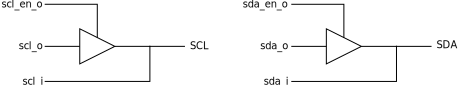
\includegraphics[width=.75\textwidth]{fig/i2c-ports}}
  \caption{Connecting the I$^2$C ports}
  \label{fig:i2c-ports}
\end{figure}

To instantiate a tri-state buffer in VHDL:

\footnotesize
\begin{verbatim}
      SCL   <= scl_o when (scl_en_o = '1') else
               'Z';
      scl_i <= SCL;

      SDA   <= sda_o when (sda_en_o = '1') else
               'Z';
      sda_i <= SDA;
\end{verbatim}

\normalsize
\noindent and in Verilog:

\footnotesize
\begin{verbatim}
      assign SCL   = (scl_en_o) ? scl_o : 1'bz;
      assign scl_i = SCL;
      assign SDA   = (sda_en_o) ? sda_o : 1'bz;
      assign sda_i = SDA;
\end{verbatim}

\normalsize

\begin{table}[h]
  \caption{Ports and generics of \textit{gc\_i2c\_slave} module}
  \label{tbl:ports}
  \centerline
  {
    \begin{tabular}{l p{.8\textwidth}}
      \hline
      \multicolumn{1}{c}{\textbf{Name}} & \multicolumn{1}{c}{\textbf{Description}} \\
      \hline
      g\_gf\_len & Glitch filter length generic \newline
                     1 -- glitches narrower than 1 \textit{clk\_i} cycle are filtered \newline
                     2 -- glitches narrower than 2 \textit{clk\_i} cycles are filtered \newline
                     etc.\\
      clk\_i & Clock input \\
      rst\_n\_i & Active-low reset input \\
      scl\_i & SCL line input \\
      scl\_o & SCL line output \\
      scl\_en\_o & SCL line tri-state enable \\
      sda\_i & SDA line input \\
      sda\_o & SDA line output \\
      sda\_en\_o & SDA line output tri-state enable \\
      i2c\_addr\_i & I$^2$C slave address of the module, compaired against received address \\
      ack\_i & ACK to be sent to the master in case of master write transfers \newline
                   '1' -- send an ACK to the master (ACK bit = '0') \newline
                   '0' -- send an NACK to the master (NACK bit = '1') \\
      tx\_byte\_i & Byte of data to be sent over I$^2$C \\
      rx\_byte\_o & Byte received over I$^2$C \\
      sta\_p\_o   & Start condition on I$^2$C bus (one-cycle-wide pulse) \\
      sto\_p\_o   & Stop condition on I$^2$C bus (one-cycle-wide pulse) \\
      addr\_good\_p\_o & Slave address received from master corresponds that on
                             i2c\_addr\_i (one-cycle-wide pulse) \\
      r\_done\_p\_o & Slave read done (one-cycle-wide pulse) \\
      w\_done\_p\_o & Slave write done (one-cycle-wide pulse) \\
      op\_o & State of the R/W bit at the end of the address byte \\
      \hline
    \end{tabular}
  }
\end{table}

\pagebreak
The rest of the ports should be connected in a normal manner to an external controlling module. A
component declaration of the \textit{gc\_i2c\_slave} module is readily available in the
\textit{gencores\_pkg.vhd} file.

%==============================================================================
% SEC: I2C bus
%==============================================================================
\section{I$^2$C Bus Protocol}
The I$^2$C bus protocol is a two-wire protocol defined by Philips/NXP. The original 
specification \cite{i2c-spec} defines all aspects of the protocol, from hardware 
connections on the bus, to bit- and byte-level data transfers and electrical
characteristics of the bus. A summary of the protocol is given here.

\begin{figure}[h]
  \centerline{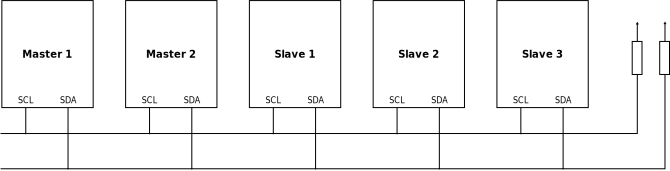
\includegraphics[width=\textwidth]{fig/i2c-bus}}
  \caption{I$^2$C bus topology}
  \label{fig:i2c-bus}
\end{figure}

Devices on the I$^2$C bus are connected together via two pins on the bus: the SCL 
(serial clock) and SDA (serial data) pins. I$^2$C masters drive the SCL line to send or
receive bits on the SDA line. Both the SCL and SDA lines on an I$^2$C device are open-collector
pins; as Figure~\ref{fig:i2c-bus} shows, one pull-up resistor on the bus connects the line to 
VCC and I$^2$C devices connect the SCL and SDA lines to ground when they drive the lines. 
In this way, a device can set a logic low level on the bus by driving the pin and a logic 
high level by releasing the pin.

A typical I$^2$C bit-level transfer (Figure~\ref{fig:i2c-bitlevel}) follows the following sequence:
\begin{itemize}
  \item master sends a start condition, driving the SDA line low while the SCL line is high
  \item master issues a series of SCL pulses to a slave to read or write bits;
  the SDA line must be stable for the duration of SCL high pulse for the bit to be properly
  transferred
  \item master sends a stop condition by releasing the SDA line while SCL line is high,
  or a repeated start (similar to start) condition if it wants to continue data transfer
\end{itemize}

\begin{figure}[h]
  \centerline{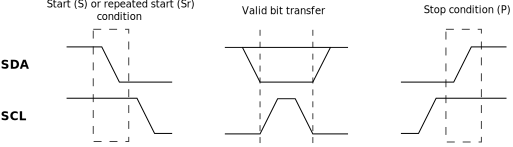
\includegraphics[width=.9\textwidth]{fig/i2c-bitlevel}}
  \caption{Bit-level transfers on the I$^2$C bus}
  \label{fig:i2c-bitlevel}
\end{figure}

Data are transferred on the bus in bytes, one bit at a time starting with the most significant bit.
After each sent byte, the other communicating party ACKs~('0') or NACKs~('1') the transfer on a
9$^{th}$ SCL cycle. Any number of bytes can be sent during a transfer, the master decides when data
transfer should stop by sending the stop condition. The folowing steps comprise a complete I$^2$C
data transfer (Figure~\ref{fig:i2c-transf}):
\begin{itemize}
  \item master sends start condition
  \item master sends slave address (7 bits of address + one R/W bit)
  \item if a slave with this address exists, it ACKs ('0') the master
  \item based on the R/W bit ('0' for read from  slave, '1' for write to slave), the master either
  reads or writes a byte bit by bit from/to the slave
  \item the receiver ACKs ('0') or NACKs ('1') the byte on the ninth SCL cycle
  \item any number of bytes may be sent, each followed by an ACK or NACK from the receiver
  \item \textbf{optional:} the master may (or may not) reverse data transfer by issuing a repeated start and sending the
  slave address with the R/W bit flipped
  \item \textbf{optional:} any number of bytes may be sent, each followed by an ACK or NACK from the receiver
  \item the master ends data transfer by sending the stop condition
\end{itemize}

\begin{figure}[h]
  \centerline{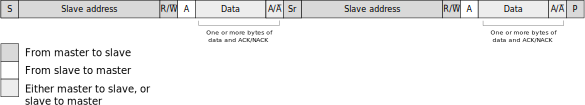
\includegraphics[width=\textwidth]{fig/i2c-transf}}
  \caption{Bytes transferred on the I$^2$C bus}
  \label{fig:i2c-transf}
\end{figure}

%==============================================================================
% SEC: Operation
%==============================================================================
\pagebreak
\section{Operation}
\label{sec:oper}

The \textit{gc\_i2c\_slave} waits for a start condition to be performed on the I$^2$C bus by a
master module. The address is shifted in and if it matches the slave address set via 
the \textit{i2c\_addr\_i} input, the \textit{addr\_good\_p\_o} output is set for one
\textit{clk\_i} cycle Based on the eighth bit of the first I$^2$C transfer byte, the module
then starts shifting in or out each byte in the transfer, setting the the \textit{r\_done\_p\_o}
pin high for one \textit{clk\_i} cycle after each successfully read byte, and respectively
the \textit{w\_done\_p\_o} output after each successfully written byte.

The \textit{ack\_i} port is used for sending the ACK to the master. The polarity of the bit
is opposite to that of the I$^2$C ACK signal. On the I$^2$C bus, a '0' signals an ACK while a '1'
an NACK. To send an ACK, the user sohuld input a '1' on the \textit{ack\_i} port. 

Note that a '1' should be set at the input also when the address is ACKed, otherwise the slave
will not acknowledge its own  address. NACKing the slave address can be used when the user
wants to isolate the slave from the bus.

Additionally, the slave module includes two one-cycle-wide pulse ports (\textit{sta\_p\_o} and
\textit{sto\_p\_o}), which signal when a start and stop condition occurs on the bus.

%------------------------------------------------------------------------------
\subsection{Read mode}

When the eighth bit of the address byte is low (R/W = '0'), the slave goes into read
mode. Each bit of the byte sent by the master is shifted in on the rising edge of SCL. After 
eight bits have been shifted in, \textit{r\_done\_p\_o} is set for one \textit{clk\_i}.
The received byte should be read from the \textit{rx\_byte\_o} output and an ACK~('1') or
NACK~('0') should be sent to the master via the \textit{ack\_i} pin. The \textit{gc\_i2c\_slave}
module does not implement clock stretching, so the \textit{ack\_i} pin should be set before
the SCL line goes high.

The steps below should be followed when reading one or more bytes sent by the master:

\begin{enumerate}
  \item Wait for \textit{addr\_good\_p\_o} to go high, signaling the I$^2$C address of the slave
    has been read.
  \item Check that that \textit{op\_o} is '0' (master write, slave read). Set a '1' at the
  \textit{ack\_i} input to send the ACK to the address; if \textit{ack\_i} is set '0', the slave
    does not acknowledge its own address.
  \item Wait for \textit{r\_done\_p\_o} to go high.
  \item Read the received byte from \textit{rx\_byte\_o} and write a '1' at \textit{ack\_i}
    to send an ACK, or a '0' to send an NACK.
  \item The transfer is repeated until the master sends a stop condition.
  \item After the stop condition is received, \textit{sto\_p\_o} goes high for one \textit{clk\_i}
    cycle and the slave goes idle.
\end{enumerate}

Note that on start conditions, \textit{sta\_p\_o} is set high for one \textit{clk\_i} cycle.

%------------------------------------------------------------------------------
\subsection{Write mode}

When the slave is to write to the master, the eighth bit of the address byte is high
(R/W = '1'). In this case, the \textit{gc\_i2c\_slave} module goes in write mode, where
the byte at the \textit{tx\_byte\_i} port is sent to the master. When the byte has been
successfully sent, the \textit{w\_done\_p\_o} is high for one clock cycle, signaling the
slave has successfully sent a byte and is awaiting the loading of another byte.

The steps below should be followed when writing one or more bytes to a master:

\begin{enumerate}
  \item Wait for \textit{addr\_good\_p\_o} to go high, signaling the I$^2$C address of the slave
    has been read.
  \item Check that \textit{op\_o} is '1' (master read, slave write). Set the byte to be sent
    to the master at the \textit{tx\_byte\_i} input. Set a '1' at \textit{ack\_i} to send the
    ACK to the address; if \textit{ack\_i} is set '0', the slave does not acknowledge its own
    address.
  \item Wait for \textit{w\_done\_p\_o} to go high.
  \item Set the next byte to be sent at the \textit{tx\_byte\_i} port.
  \item If the master acknowledges the transfer, the next byte is sent, otherwise, the master
    will send a stop condition, and the \textit{gc\_i2c\_slave} module is returned to IDLE. The
    \textit{sto\_p\_o} output is also set high for one \textit{clk\_i} cycle.
\end{enumerate}

Note that on start conditions, \textit{sta\_p\_o} is set high for one \textit{clk\_i} cycle.

%==============================================================================
% SEC: Implementation
%==============================================================================
\section{Implementation}
\label{sec:implem}

A simplified block diagram of the \textit{gc\_i2c\_slave} module is presented in
Figure~\ref{fig:i2c-slave-bd}. Deglitched versions of the SCL and SDA lines control
operation of the central finite-state machine (FSM), which sets the outputs and
controls the rest of the components in the module. The glitch filter lengths can
be set in units of \textit{clk\_i} cycles via the \textit{g\_gf\_len} module generic.
The FSM controls how outputs are set, when the reception and transmission shift registers
(RXSR/TXSR) are loaded and when they shift, and acknowledging to the address and bytes
sent by the master.

\begin{figure}[h]
  \centerline{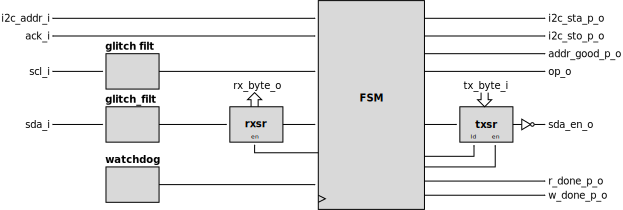
\includegraphics[width=\textwidth]{fig/i2c-slave-bd}}
  \caption{Block diagram of \textit{gc\_i2c\_slave} module}
  \label{fig:i2c-slave-bd}
\end{figure}

Figure~\ref{fig:fsm-diag} shows a simplified state transition diagram of the FSM,
and Table~\ref{tbl:fsm} lists the states of the FSM and the operations performed in each
state. Across the FSM, shifting of bits into the module is done on the rising edge
of SCL and shifting out is done on the falling edge of SCL. A three-bit counter is
used to count the number of bits that are sent and received by the module. This bit
counter is incremented on the rising edge of SCL. During read and write cycles, the
FSM changes states on the SCL falling edge. A summary of the FSM actions with
reference to the SCL line on read and write transfer is shown in
Figure~\ref{fig:fsm-and-scl}.

\begin{figure}[h]
  \centerline{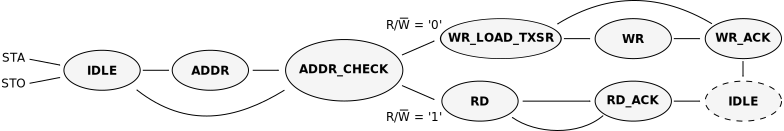
\includegraphics[width=\textwidth]{fig/fsm-diag}}
  \caption{Simplified FSM state transition diagram}
  \label{fig:fsm-diag}
\end{figure}

\begin{figure}[h]
  \centerline{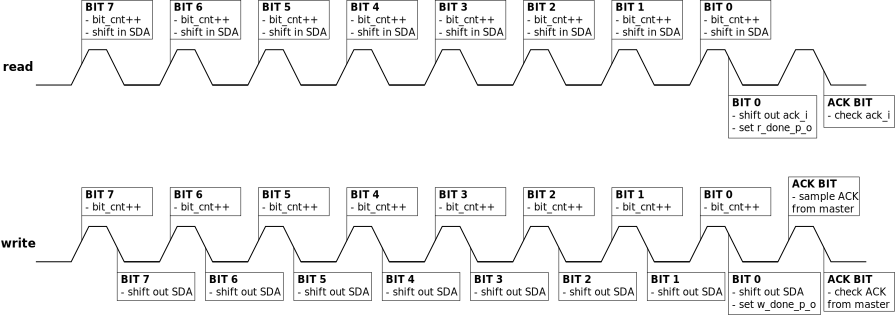
\includegraphics[width=\textwidth]{fig/fsm-and-scl}}
  \caption{FSM actions on SCL edges}
  \label{fig:fsm-and-scl}
\end{figure}

\begin{longtable}{l p{.7\textwidth}}
  \caption{The states of the \textit{gc\_i2c\_slave} FSM}
  \label{tbl:fsm} \\

    \hline
    \multicolumn{1}{c}{\textbf{State}} & \multicolumn{1}{c}{\textbf{Description}} \\
    \hline
    \endfirsthead
    
    \hline
    \multicolumn{1}{c}{\textbf{State}} & \multicolumn{1}{c}{\textbf{Description}} \\
    \hline
    \endhead
    
    \hline
    \endfoot
    
    \textit{IDLE} & Default state after reset and the state returned to after
                    reception of a start and stop condition. \\
    \textit{ADDR} & Shift in the address and R/W bit. \\
    \textit{ADDR\_ACK} & Send ACK depending on value of \textit{ack\_i} and go to \textit{RD} state
                         if the R/W bit is high, or to \textit{WR\_LOAD\_TXSR} state if R/W bit is low.
                         If \textit{ack\_i} is low, go back to \textit{IDLE}. \\
   \textit{RD} & Shift in eight bits sent by master and go to \textit{RD\_ACK} state. Each bit 
                 is shifted in on the rising edge of SCL. \\
    \textit{RD\_ACK} & Send ACK depending on value of \textit{ack\_i}. If \textit{ack\_i} is '1',
                       then go back to \textit{RD} state, else to \textit{IDLE} state. \\
    \textit{WR\_LOAD\_TXSR} & Load TX shift register with data at \textit{tx\_byte\_i} input
                              and go to \textit{WR} state. \\
    \textit{WR} & Shift out the eight bits of the TXSR starting with MSB and go to 
                  \textit{WR\_ACK} state. TXSR shifts left on each falling edge of SCL. \\
    \textit{WR\_ACK} & Read ACK bit sent by master. If '0', go back to \textit{WR} state, otherwise
                       go to \textit{IDLE} state. \\
\end{longtable}

%------------------------------------------------------------------------------
\subsection{Output control}

To keep to the I$^2$C standard, the I$^2$C outputs (\textit{sda\_o}, \textit{scl\_o}) are
not directly driven high. Instead, they are driven low and their respective enable outputs
are driven high and low, to enable the output buffers. In fact, since no clock stretching
is implemented, the SCL line is always disabled.

Therefore, when the term "send" is used below, it means controlling the \textit{sda\_en\_o}
line high and low to enable the output buffer and send a '0', or leave the line high.

%------------------------------------------------------------------------------
\subsection{Address byte}

The transfer starts by the master sending a start condition on the I$^2$C bus.
The slave detects this start condition and starts shifting in the address bits while in the
\textit{ADDR} state. After the eighth bit has been shifted in, the FSM goes into the
\textit{ADDR\_CHECK} state, where it checks the received address versus the
\textit{i2c\_addr\_i} pin and if it matches, the FSM goes into the \textit{ADDR\_ACK} state,
where the slave waits for the \textit{ack\_i} input to be set by the external controller.

If the external controller sets the \textit{ack\_i} pin high while the slave is
in the \textit{ADDR\_ACK} state, the slave module acknowledges its address received
from the master, and the transfer continues as indicated by the eighth bit in the
address byte.

While in the \textit{ADDR\_CHECK} state, the \textit{op\_o} and \textit{addr\_good\_p\_o}
outputs are also set high (\textit{addr\_good\_p\_o} is set for one clock cycle and
\textit{op\_o} is set until the next I$^2$C transfer).

Important to note is that if the address received from the master does not correspond
to \textit{i2c\_addr\_i} when it is checked in the \textit{ADDR\_CHECK} state, the
slave module NACKs the transfer and goes back to the \textit{IDLE} state, setting an inhibit
signal. The purpose of this inhibit signal is to prevent the slave from reacting to
other bytes sent by a master to another slave on the I$^2$C bus. If this inhibit
signal were not present and if a byte sent by the master to another slave on the bus
matches the slave module's address at the \textit{i2c\_addr\_i} port, the slave module
would acknowledge this byte as its own address. The inhibit signal is cleared only when
receiving a start or a stop condition, as after one of these two, the master would
send the I$^2$C slave address again, and this is when the slave module should become
active again.

%------------------------------------------------------------------------------
\subsection{Reading from a master}

The slave will read from a master when this eighth bit is high ('1'). On read
transfers, the FSM is in the \textit{RD} state, where bits on the SDA line are shifted
in by the slave on the rising edge of SCL (see Figure~\ref{fig:fsm-and-scl}). This
happens until the eighth bit has been shifted in, at which point the \textit{r\_done\_p\_o}
pin is set for one clock cycle and the FSM goes into the \textit{RD\_ACK} state. Here,
the external module controls the \textit{ack\_i} pin to ACK/NACK the received byte,
as in the case of the \textit{ADDR\_ACK} state. If the external module ACKs the
transfer, the slave module goes back to the \textit{RD} state to read another byte
from the master, or to the \textit{IDLE} state otherwise.

%------------------------------------------------------------------------------
\subsection{Writing to a master}

The slave will write to a master when the eighth bit in the address byte is low ('0').
On write transfers, the FSM is in the \textit{WR} state, where bits on the SDA line
are shifted out of the slave on the falling edge of SCL (see Figure~\ref{fig:fsm-and-scl}).
This happens until the eight bit has been transferred, at which point the slave sents
the \textit{w\_done\_p\_o} pin for one clock cycle and it goes into the \textit{WR\_ACK}
state, where it waits for the master to acknowledge the sent byte. The ACK from the master
is sampled in on the rising edge of SCL and it is checked on the falling edge of SCL,
to determine whether a new write transfer should occur or not. If the master has
ACKed the transfer, the FSM goes back to the \textit{WR} state to send another byte to
the master, or to the \textit{IDLE} state otherwise.

%------------------------------------------------------------------------------
\subsection{Start and stop conditions on the bus}

A start or a stop condition will take the slave module back into the \textit{IDLE}
state, irrespective of other control signals internal to the module.

The inhibit signal is also cleared on these two conditions, as the master would
follow up by sending an address byte relevant to the slave module.

%==============================================================================
% Bibliography
%==============================================================================
\pagebreak
\bibliographystyle{ieeetr}
\bibliography{gc_i2c_slave}

\end{document}
